\documentclass{sig-alternate}
%
%\usepackage{makeidx}  % allows for indexgeneration
%\usepackage[pdftex]{graphicx}\usepackage{graphicx}
\usepackage{float}
\usepackage{subfig}
\usepackage{caption}
\DeclareCaptionType{copyrightbox}
\usepackage{graphicx}
\usepackage{amsmath}
\usepackage{algorithm,algorithmicx}
\usepackage{algpseudocode}

\begin{document}
%\normalem


\title{Why so aggressive? Low Extra Delay Backround Traffic (LEDBAT) in WebRTC}

\numberofauthors{3}

\author{
\alignauthor
Riccardo Reale\\
      \affaddr{Peerialism AB}\\
      \affaddr{Stockholm, Sweden}\\
      \email{riccardo@peerialism.com}
\alignauthor
Anton Blomberg\\
      \affaddr{Stockholm University}\\
      \affaddr{Stockholm, Sweden}\\
      \email{anton@su.se}
\alignauthor
Roberto Roverso\\
      \affaddr{Peerialism AB}\\
      \affaddr{Stockholm, Sweden}\\
      \email{roberto@peerialism.com}
}

\newcommand{\mysec}[1]{\vspace*{-0.0cm}\section{#1}}
\newcommand{\mysubsec}[1]{\vspace*{-0.0cm}\subsection{#1}\vspace*{0cm}}
\newcommand{\mysubsubsec}[1]{\vspace*{-0.0cm}\subsubsection{#1}\vspace*{0cm}}
\newcommand{\mypar}[1]{\vspace*{-0cm}\paragraph{#1}\vspace*{0cm}}

\maketitle
%\vspace*{-1cm}

\begin{abstract}

In this paper, we present what is, to the best of our knowledge, the first implementation
of LEDBAT for the WebRTC framework. In particular, we detail how we integrated the
protocol in the WebRTC stack in a way that features such as reliability, in-order
delivery and encryption \textbf{ (NAT?)} could also be applied to LEDBAT transfers and not only to
the existing transfer protocol (SCTP). We also include preliminary results of this effort
that show the correct functioning of our implementation.
\end{abstract}

\category{C.2.2}{Computer-Communication Networks}{Network Protocols}
\category{C.2.4}{Computer-Communication Networks}{Distributed Systems}
\terms{Experimentation, Performance, Measurement}
\keywords{LEDBAT, WebRTC, Peer-to-peer}

\mysec{Introduction}
% WebRTC general 
Recently, WebRTC has been steadily gaining popularity fueled by the inclusion in most of
the browsers on the market. The WebRTC standard mandates the multimedia and peer-to-peer
connectivity stacks for real-time services, once provided by external plugins, to be built
directly into the browser. That means that the functionality of those stacks, such as
video acquisition, noise cancelling and NAT traversal, is directly available through
Javascript and HTML5 APIs. Although WebRTC has been mainly designed as a framework to
facilitate video and audio conferencing, it does include support for building other types
of peer-to-peer applications, such as CDN accellerators~\cite{peerCDN} and video streaming
platforms~\cite{nurminen2013p2p}. This feature is provided through the DataChannel
abstraction, which allows the transfer of arbitrary data over encrypted connections
established with WebRTC's NAT traversal facilities. The DataChannel API make use of the
Stream Control Transfer protocol (SCTP)~\cite{sctp} protocol in order to manage data
transfers. SCTP is message-oriented protocol and provides a variety of options on data
transfer to accomodate the needs of different types of applications. When setting up a
DataChannel, WebRTC applications may choose in- or out-of-order delivery, reliable or
unreliable delivery and have a specific priority level on the channel. Regarding
congestion control, the latest version of SCTP included in WebRTC make use of the same
congestion control found in H-TCP~\cite{htcp}. The main characteristic of H-TCP is that it
delivers the same priority as TCP in low bandwidth networks while trying to better exploit
High Delay-Bandwidth Product links always compared to TCP.

% Why LEDBAT is important
Although the DataChannel implementation currently provides very useful features, it lacks
a fundamental component that is background traffic. This is usually provided in P2P
network stacks by a delay-based congestion control protocol such as LEDBAT~\cite{ledbat}. 
LEDBAT achieves low priority behaviour by completely yielding to other TCP traffic on the same
network and by keeping the delay on a link fixed to a low and constant target. By adopting
such protocol, data-intensive applications such as Bittorrent avoid disrupting both
TCP-based web browsing and low delay VoIP applications. Low priority traffic is also a
vital requirement for other types of applications, such as streaming
platforms ~\cite{smoothcache}\cite{roberto-thesis}.

% What we did 
In this paper, we present what is, to the best of our knowledge, the first implementation
of LEDBAT for the WebRTC framework. In particular, we detail how we integrated the
protocol in the WebRTC stack such that features like encryption and NAT traversal could also 
be applied to LEDBAT transfers and not only to SCTP. We also include
preliminary results of this effort that show the correct functioning of our
implementation.

% Open source
The implementation is open-source and can be found at~\cite{}. We hope that, by adding
LEDBAT to WebRTC, we will enable a new class of data-intensive applications to be
developed on Javascript that are pluginless and can coexist with standard web browsing
and the typical application of WebRTC, that is conferencing.



\begin{figure}[t]
  \centering
    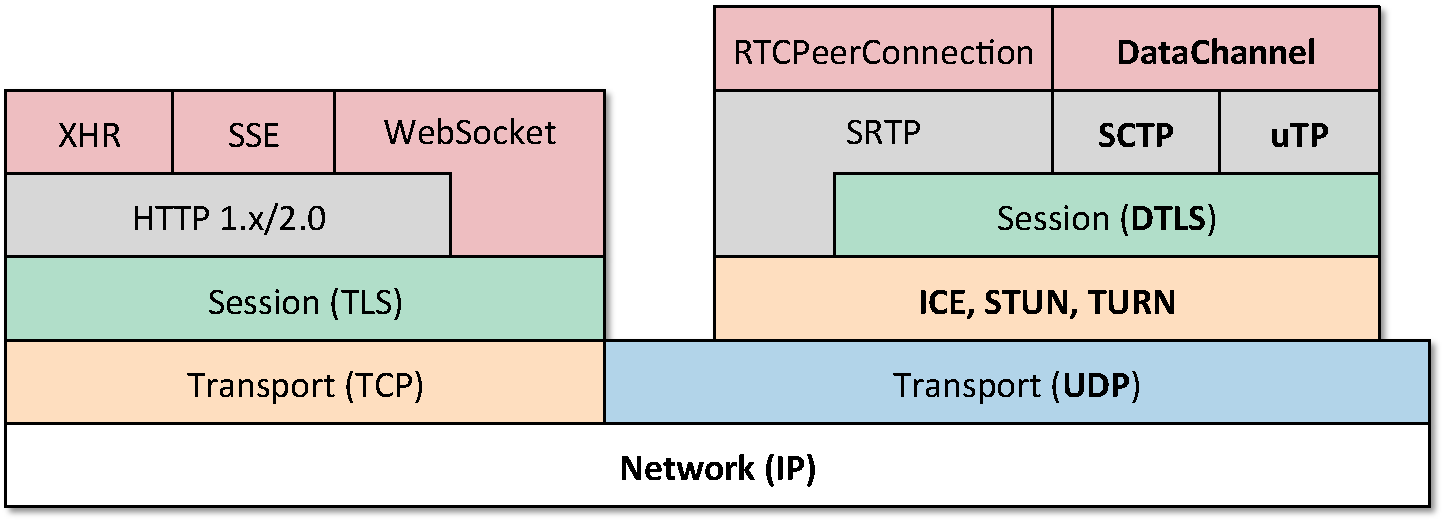
\includegraphics[width=0.46\textwidth]{figs/architecture2}
\vspace*{-0.38cm}
	\caption{WebRTC protocol stack} \label{fig:architecture}
\vspace*{-0.4cm}
\end{figure}

\mysec{LEDBAT in WebRTC}

% - how SCTP work
%The main reason why SCTP was chosen as application level transport protocol for the DataChannel is that it natively support some interesting features such as configurable in-order delivery, configurable reliability and a channel priority level defined by the application. Moreover it provides flow control and congestion control, while security is ensured by tunnelling all the traffic through a secure DTLS session, which itself run on top of UDP.
The WebRTC DataChannel currently includes a user-level SCTP library [?] written in \textit{C} and built on top of UDP. Moreover all the traffic is tunnelled through a secure DTLS session, to ensure confidentiality and integrity of the transferred data.

% - what we changed
In order to implement LEDBAT support in WebRTC we decided to directly integrate the \textit{uTP} library \cite{utp-repo} in the DataChannel protocol stack as an alternative to the SCTP one. uTP is the open-source BitTorrent implementation of LEDBAT which also provides reliability and in-order delivery. The library is built on top of UDP, and therefore it can make use of the remaining existing DataChannel protocol stack, included DTLS and the NAT-traversal component. The DataChannel API has been therefore modified to be able to choose between SCTP and uTP as transport protocol to use when setting up a data channel between two WebRTC instances. In Figure \ref{fig:architecture} is shown the resulting WebRTC protocol stack.

% - shortcomings
The DataChannel transport protocol selection is not yet supported by the W3C standard Javascript API, therefore we developed a test application in \textit{C} that generates traffic using directly the WebRTC Native DataChannel API to emulate the traffic generated by a data-intensive browser application.

\label{sec:architecture}

\mysec{Preliminary results}

% - setup
We conducted a preliminary evaluation of our solution in a controlled network environment consisting of two host machines, a sender and a receiver, running Linux Ubuntu with kernel 3.11.0-12 connected through a 100 Mbit/s link. We used Dummynet on the sender host, configured to cap the outgoing traffic to 1Mbps, with 100 ms base delay and 60KB of queue buffer to simulate a typical WAN gateway scenario. Both hosts run our test application and a separate TCP traffic generator to obtain traffic competing on the same network resources. The browser emulator can be configured to initialize either a STCP DataChannel, or a LEDBAT DataChannel, while the TCP file transfer uses TCP Cubic, the default Linux congestion control. Finally a third host acts as a server to handle the WebRTC session signalling between the sender and the receiver.

% - metrics
As metrics to evaluate the uTP library integration we measured the throughput of the generated DataChannel LEDBAT streams competing against a TCP one and the Round Trip Time (RTT) on the bottleneck link. The rationale behind this experiment is to verify the correct behaviour of the LEDBAT congestion control in the presence of higher priority traffic insisting on the same bottleneck, and, at the same time, analyse the relative increase on the one-way delay, which directly affects latency and, therefore, web browsing responsiveness. 

% - evaluation
Figure \ref{fig:2ledbat_tcp} shows the throughput evolution of two DataChannel LEDBAT streams and a single TCP, starting at 60 seconds distance each, and the correspondent Round Trip Time. The two LEDBAT flows correctly show a background traffic behaviour, using all the available network resources while quickly releasing them in favour of the higher priority TCP flow. The increase in the RTT due to LEDBAT flows is limited to 100 millisecond, which is the default target delay configuration in uTP. Note that the number of LEDBAT streams doesn't affect the amount of extra delay introduced.

%During the initial two minutes of the experiment, the LEDBAT streams correctly use all the available network resources while maintaining the introduced extra delay to a maximum of 100 millisecond, correspondent to the default target delay configured in uTP. At second 120 the two streams quickly release resources in favour of the higher priority TCP flow until it terminates. 

For direct comparison, figure \ref{fig:2sctp_tcp} shows the same experiment performed configuring our test application to use DataChannel SCTP streams. Besides fairly sharing the link with the TCP flow as expected, each of the SCTP streams introduce a large amount of extra-delay on the link.

% - conclusion
In conclusion, the extra-delay introduced by data-intensive WebRTC application may have strong repercussion on latency-sensible experiences such as web browsing or conferencing, and we recommend the introduction of LEDBAT to overcome this problem.

\begin{figure}[t]
  \centering
    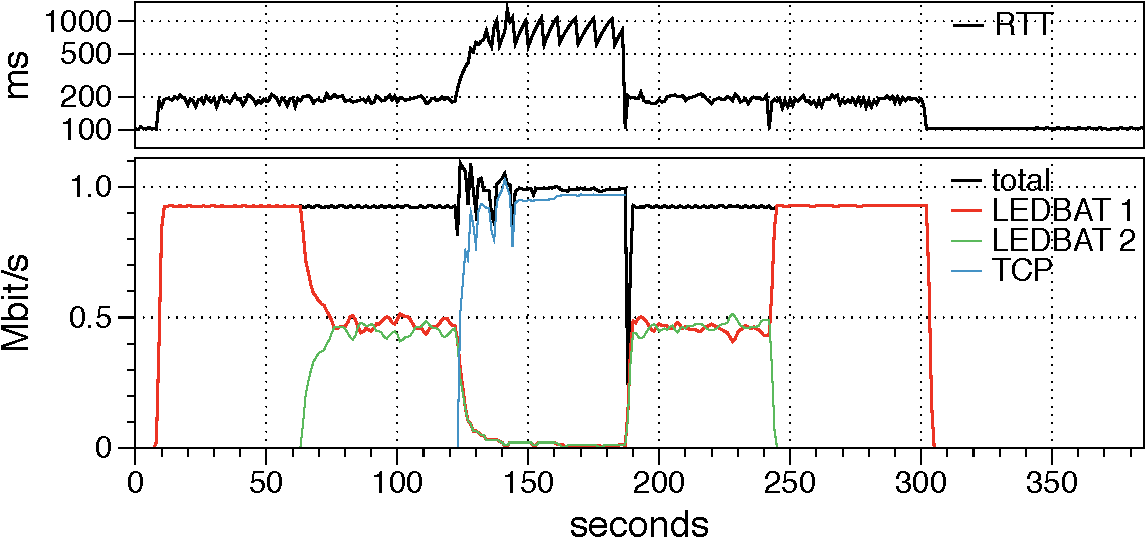
\includegraphics[width=0.47\textwidth]{figs/2ledbat_tcp}
\vspace*{-0.38cm}
	\caption{Two DataChannel LEDBAT streams sharing a 1Mbit/s bottleneck with a TCP stream} \label{fig:2ledbat_tcp}
\vspace*{-0.4cm}
\end{figure}

\begin{figure}[t]
  \centering
    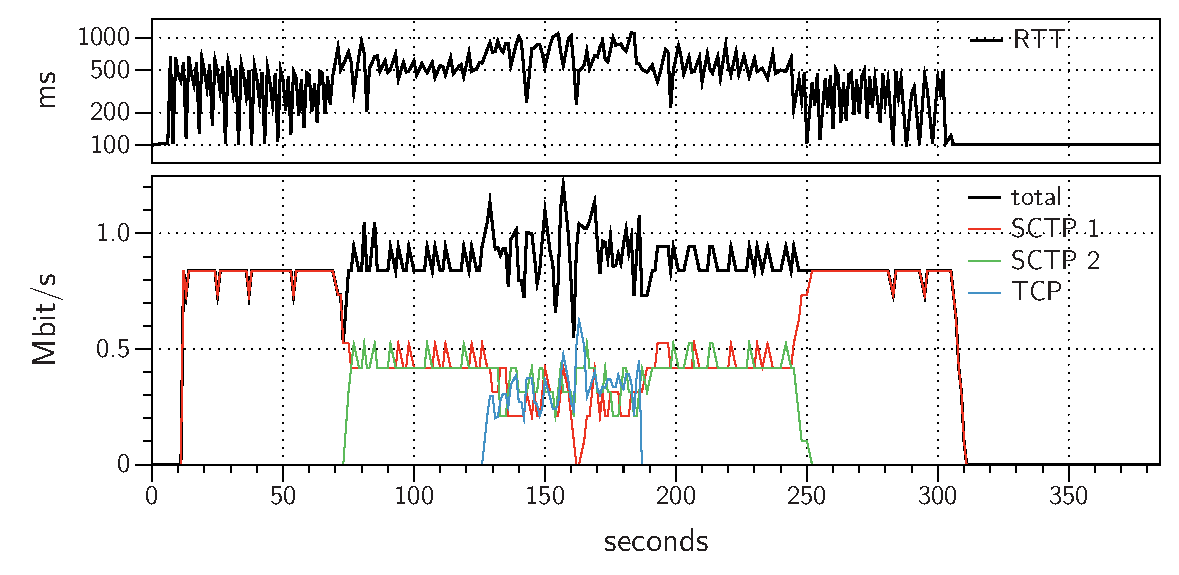
\includegraphics[width=0.47\textwidth]{figs/2sctp_tcp}
\vspace*{-0.38cm}
	\caption{Two DataChannel SCTP  streams sharing a 1Mbit/s bottleneck with a TCP stream} \label{fig:2sctp_tcp}
\vspace*{-0.4cm}
\end{figure}

\bibliographystyle{abbrv}
\bibliography{main}


\end{document}
